\chapter{The Generalization of \ac{ros2} Interface for Webots}
\label{chap:generalization}
\shorttitle{\nameref{chap:generalization}}


\section{Introduction}
\label{sec:generalization:introduction}

Up to now, the \ac{ros2} interface for the e-puck2 robot in Webots has been created manually.
It means that the Webots controller has to be written to expose \ac{ros2} interfaces.
Although this method gives a developer much flexibility, it is time demanding, prone to errors, and requires changes every time the Webots robot model is alternated.
Since the Webots model is accessible from the Webots \ac{api}, we saw an opportunity to automate the process of creating \ac{ros2} driver for Webots.

% objectives (hybrid)
The primary objective is to create a universal launch file that is supposed to read the Webots robot model and create \ac{ros2} interface accordingly.
This process has to be fully automated by default, highly configurable, and it has to work in conjunction with the user's custom code.
The universal launch file allows users to bootstrap the project and benefit from reusable blocks quickly, furthermore, it also offers a possibility to configure the \ac{ros2} interface and extend the driver if needed.

% pros and cons
This system is supposed to bring a few major advantages for the users, the most important of which is the reduction of development time.
Instead of writing a custom Webots controller, which exposes the \ac{ros2} interface for each robot, the process of creating a \ac{ros2} interface can be completely avoided reducing development time significantly.
Besides, if the controller written by the user is not implemented properly, every iteration on the model requires changes in the controller.
For example, if \texttt{lookupTable} field of \texttt{DistanceSensor} is changed in model, the controller should be updated accordingly.
The second major advantage of the universal driver is that it is less prone to errors.
Since the universal driver is supposed to be maintained by the Webots team and community, the bugs should be discovered and fixed quickly.
However, the universal driver and launch introduce a level of abstraction hiding implementation details and customization possibilities.
Therefore, the building blocks must be carefully designed to allow a high level of customization if needed.

% challenges
As mentioned, the universal driver needs access to the Webots robot model to generate a proper \ac{ros2} interface.
This will present multiple challenges:
if a Webots robot is not configured to work as Supervisor, many aspects of Webots robot model are hidden.
Therefore, the Webots controller \ac{api} has to be extended, the most importantly, the \ac{api} needs to be extended to support allow \ac{ros2} transforms.
The other missing functions in the Webots \ac{api} is, for example, access to a lookup table of \texttt{DistanceSensor}.
The access to lookup table is needed because the \texttt{sensor\_msgs/Range} topic requires real values to be published instead of raw values.



\section{Design}

% In the previous section, the idea of Webots to \ac{ros2} interface generalization is presented, focusing on the objective, advantages, and challenges.
In this section, more details on the design will be given. Nevertheless, we need to review the approach that has taken place up to now (see Figure \ref{fig:generalization:ros2_driver_within_webots}). 

% https://docs.google.com/drawings/d/1hRj3ivxq4uhepWZhiJNc_sa_-RWV9RomA9dyEC2PbiI/edit?usp=sharing
\begin{figure}[H]
    \centering
    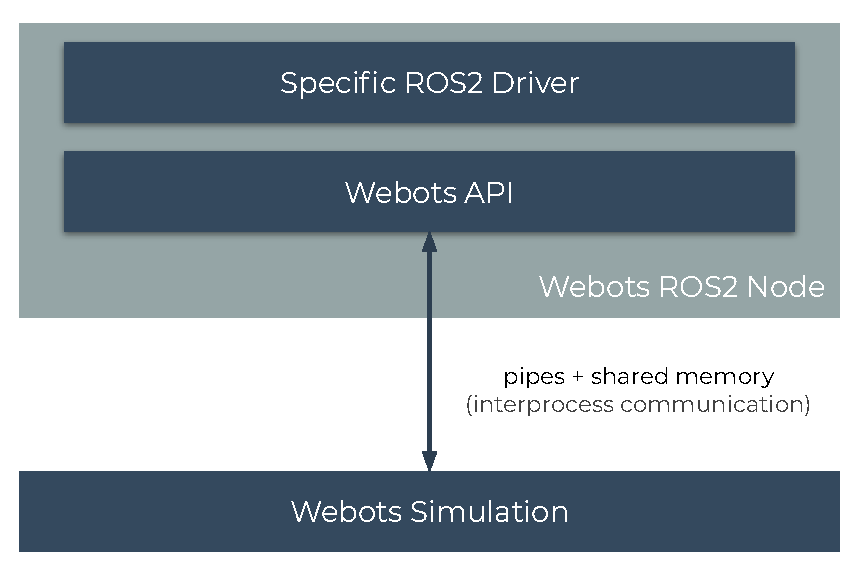
\includegraphics[width=0.8\textwidth]{generalization/figures/ros2_driver_within_webots.pdf}
    \caption{Technique of creating \ac{ros2} interface within Webots before universal driver and launch file are introduced}
    \label{fig:generalization:ros2_driver_within_webots}
\end{figure}

As shown in the picture, the process of creating \ac{ros2} driver required of user to use Webots \ac{api} to write \ac{ros2} driver. 
The user had to write a layer that sits in between low-level \ac{api} (Webots \ac{api} in this case) and \ac{ros2} interface. 
Although this is a necessary step for the real robots and allows users a lot of customization (or even ability to optimize), the objective is to avoid the step for the reasons given in the previous section (see Section \ref{sec:generalization:introduction}).

Therefore, the new universal driver design is given in the following picture.
\begin{figure}[H]
    \centering
    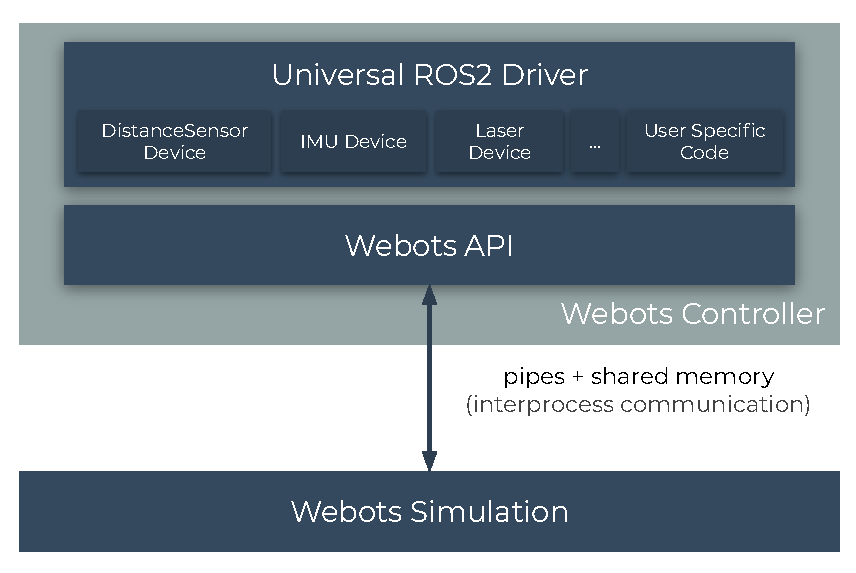
\includegraphics[width=0.8\textwidth]{generalization/figures/universal_driver_within_webots.pdf}
    \caption{Webots and \ac{ros2} interface using the new universal driver}
    \label{fig:generalization:universal_driver_within_webots}
\end{figure}

With the universal driver, a notion of devices is introduced.
A device\footnote{Note that "device" is related to a module in the universal driver and "Webots device" is a node that represents a robot device in Webots.}, in this context, represent a module which transforms data from of one or more Webots devices to one or more \ac{ros2} topics and services.
By default, the universal driver will go through all Webots devices available in a robot and try to match them with a suitable device.
If the match is found, a new device is instantiated, a Webots device is assigned to it, and the device will start publishing or subscribing to the \ac{ros2} messages.

All devices are configurable, meaning that they will use default parameters if custom parameters are not supplied.
Since a device can be parameterized from multiple sources, the priority is the following:
\begin{itemize}
    \item A parameter value obtained through \ac{ros2} parameters has the highest priority, and it will override parameter values obtained through any other source.
    \item Python dictionary consisted of parameters passed to the device manager is the second in the priority list.
    \item Default or autogenerated values have the least priority. The autogenerated values are usually based on Webots' device names.
\end{itemize}

If a user is not satisfied with the customization achieved by using the parameters, the user can write custom code for it.
A good example is distance sensors in e-puck2.
The e-puck2 has nine distance sensors positioned around the robot that could emulate \ac{lidar} and publish data to the \texttt{LaserScan} topic.
Allowing something like this in the universal driver would be too much work, and little gain due to the small number of users who would benefit from it.
Therefore, users can disable the ROSification of Webots distance sensors and implement a custom code that will publish measurements to \texttt{LaserScan} topic\footnote{The described example is implemented, explained in more details and it is publicly available.}.

\section{\ac{ros2} Transformations}

In context of \ac{ros2}, transforms represent translation and rotation between two coordinate frames (see Figure \ref{fig:generalization:tf2_robot}).
Keeping track of the transforms is important as it can provide a relative translation and rotation of two arbitrary coordinate frames in a transforms tree at any point in time \cite{foote_tf_2013}. 
\ac{ros2} considers the transforms as a vital aspect of robotics applications.
Therefore, many \ac{ros2} packages rely on the \ac{ros2} transformations.
For example, the \texttt{slam\_toolbox} uses the transforms to find translation and rotation between \texttt{base\_link} and a link that publishes to a topic of type \texttt{LaserScan}.
This is necessary as otherwise, the \texttt{slam\_toolbox} couldn't determine the robot's position in the map.

\begin{figure}[H]
    \centering
    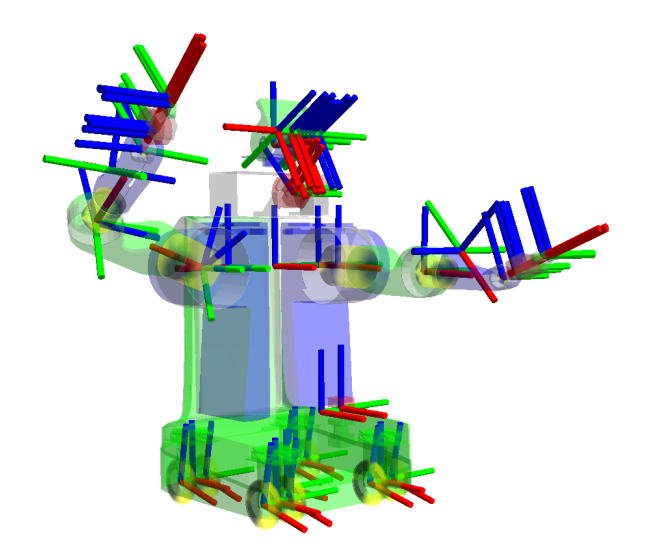
\includegraphics[width=0.8\textwidth]{generalization/figures/tf2_robot.png}
    \caption{An example of coordinate frames visualized in RViz2 \cite{foote_tf_2013}}
    \label{fig:generalization:tf2_robot}
\end{figure}

Considering the importance of transforms \ac{ros2}, the universal driver has to offer functionality to publish those transforms automatically.
To publish transforms automatically, three approaches are considered, two of which are implemented in this project's scope:
\begin{itemize}
    \item Method \#1. The absolute position of each solid node is sampled periodically and published as a dynamic transform. The whole method can be implemented in the universal driver.
    \item Method \#2. A new \ac{api} function is added to Webots, which retrieves a tree of important links and joints. The tree is parsed in the universal driver, and relative transforms are published based on corresponding encoder readings (\texttt{PositionSensor} node in Webots). 
    \item Method \#3. A new \ac{api} function is added to Webots which retrieves \ac{urdf} as a string. \ac{urdf} string is then passed to \texttt{robot\_state\_publisher} as \ac{ros2} parameter. Also, from the universal driver, encoder readings are published periodically as messages of type \texttt{sensor\_msgs/JointState}. These messages are consumed by \texttt{robot\_state\_publisher}, and corresponding transforms are published.
\end{itemize}

The following table compares the most important aspects of these methods.

\begin{table}[H]
    \centering
    \begin{tabular}{|l|c|c|c|}
        \hline
        & Method \#1 & Method \#2 & Method \#3  \\
        \hline
        Preserves noise & No & Yes & Yes \\
        \hline
        Supervisor mode is necessary & Yes & No & No \\
        \hline
        Recognizes static transforms & No & Yes & Yes \\
        \hline
        Implemented in the project scope & No & Yes & Yes \\
        \hline
    \end{tabular}
    \caption{Comparison of different methods considered for publishing \ac{ros2} transforms}
    \label{tab:generalization:transforms_comparison}
\end{table}

As shown in Table \ref{tab:generalization:transforms_comparison}, there are two significant reasons why Method \#1 is not used: it does not preserve noise that is coming from the encoders, and the robot has work in supervisor mode.
Even though the implementation does not require changes to Webots core, a considerable disadvantage is a fact that it does not preserve a realistic behavior of the robot supported in Webots.

\subsection{Transforms from \acs{urdf}}
This section describes Method \#3, which is based on exporting an \ac{urdf} document from Webots. 

\subsubsection{\acs{urdf} vs. Webots' Robot Model Representation}
However, it is important to compare \ac{urdf} format and Webots' robot model representation first.
\ac{urdf} is XML format and it uses only two primitives to describe robot model, links and joints.
There has to be at least one link defined in the URDF document, usually named as \texttt{base\_link}, and it's children can be only joints \cite{noauthor_urdf_nodate} (see Figure \ref{fig:generalization:urdf_vs_webots:urdf}).
Therefore, a link cannot be encapsulated inside another link, but can only connected with a common joint.
This is a main difference to Webots' robot representation as the root node in Webots encapsulates other nodes.
In addition to it, Webots has richer specter of nodes.
Besides the links (\texttt{Solid} node in Webots) and joints there are also nodes like \texttt{Group}, \texttt{Transform}, \texttt{Geometry} and \texttt{Shape} (see Figure \ref{fig:generalization:urdf_vs_webots:urdf}).

\begin{figure}[H]
\centering
\begin{subfigure}{.5\textwidth}
  \centering
  \inputminted{c}{generalization/data/simple.proto}
  \caption{Webots' model representation}
  \label{fig:generalization:urdf_vs_webots:webots}
\end{subfigure}%
\begin{subfigure}{.5\textwidth}
  \centering
  \inputminted[fontsize=\footnotesize]{xml}{generalization/data/simple.urdf}
  \caption{Model representation in \ac{urdf}}
  \label{fig:generalization:urdf_vs_webots:urdf}
\end{subfigure}
\caption{Typical robot representation in \ac{urdf} and in Webots of the same model}
\label{fig:generalization:urdf_vs_webots}
\end{figure}

The described two main differences in a robot model representation, hierarchy and node diversity, make \ac{urdf} export feature implementation rather complicated. 

\subsubsection{\ac{urdf} Export}
\label{subsub:generalization:urdf_export}

In this section, the main points of \ac{urdf} export feature will be described.
It is vital to know that this feature is implemented in Webots core utilizing the existing exporting robot models' mechanisms.
The mechanism already supports a robot model to be exported to \acs{vrml}, \acs{x3d} and PROTO documents.
Even though the mechanism provides useful features, flexibility to implement \ac{urdf} export is limited, and therefore the implementation may differ from what is expected in general (nodes in \ac{urdf} are related by \acs{id}, while nodes in Webots are encapsulated).

The Webots's mechanism to handle exports depends on a few methods declared in \texttt{WbNode}.
In Webots, each node is derived from \texttt{WbNode} class and in the context of \ac{urdf} export it has the following prototype:
\begin{minted}{c++}
class WbNode {
protected:
  // Calls `.writeExport()` to continue the export if needed
  virtual void write(WbVrmlWriter &writer) const;

  // Uses `WbVrmlWriter` to write node details a document
  virtual void writeExport(WbVrmlWriter &writer) const;
  
  // Uses `WbVrmlWriter` to recursively continue export (export children)
  virtual void exportNodeSubNodes(WbVrmlWriter &writer) const;
  
  // Other declarations
};
\end{minted}

Those methods have to be defined for each Webots node to write \ac{urdf} content using \texttt{WbVrmlWriter} class.
Then, the methods are recursively called from the tree root (\texttt{ robot} node) to the leaves.
To export nodes that are related by \acs{id} instead of encapsulating them is shown by the algorithm in Figure \ref{fig:generalization:urdf_flat}.

\begin{figure}[H]
    \begin{minipage}{\linewidth}
    \begin{procedure}[H]
        \tcc*{$ N_{current} $ and $ N_{queue} $ are global variables. $ N_{current} $ represent a reference on instance of \texttt{WbNode}, while $ N_{queue} $ is a queue of the references}
    
        \If{$ N_{current} \neq $ \texttt{this} $ \land $ \texttt{this} is not joint $ \land $ \texttt{this} is not in $ N_{queue} $}{
            add \texttt{this} to $ N_{queue} $  \;
        }
        
        \If{$ N_{current} $ is not set}{
            $ N_{current} $ = \texttt{this} \;
        }
        
        writeExport(\texttt{this}) \;
        
        \If{$ N_{current} $ = \texttt{this}}{
            \eIf{$ N_{queue} $ not empty}{
                $ N_{current} $ = dequeue the last node from $ N_{queue} $ \;
                write(\texttt{this}, \texttt{writter}) \;
            }{
                $ N_{current} $ = \texttt{NULL} \;
            }
        }
        \caption{write (\texttt{this}, \texttt{writter})}
    \end{procedure}
    \end{minipage}
    \begin{minipage}{\linewidth}
    \begin{procedure}[H]
        \If{$ N_{current} $ = \texttt{this}}{
            write URDF of link \;
        }
        \caption{writeExport (\texttt{this})}
    \end{procedure}
    \end{minipage}
\caption{Approach used to handle \ac{urdf}'s flat nature in object-oriented architecture}
\label{fig:generalization:urdf_flat}
\end{figure}

Properly implementing \texttt{writeExport()} to Webots' nodes that represent joints and links will produce a desired \ac{urdf} document.
However, let consider a very simple example in Figure \ref{fig:generalization:squashing_transforms:actual}.

\begin{figure}[H]
\centering
\begin{subfigure}{\textwidth}
  \centering
  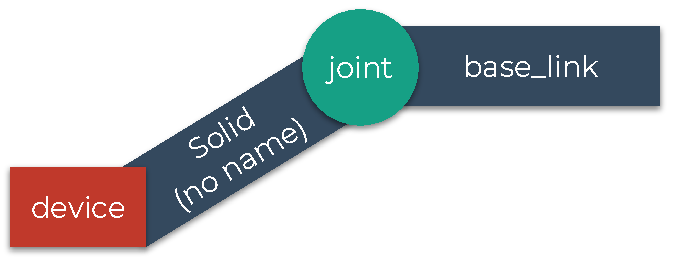
\includegraphics[width=.7\linewidth]{generalization/figures/squashing_transforms_actual.pdf}
  \caption{Exported model}
  \label{fig:generalization:squashing_transforms:actual}
\end{subfigure}
\begin{subfigure}{\textwidth}
  \centering
  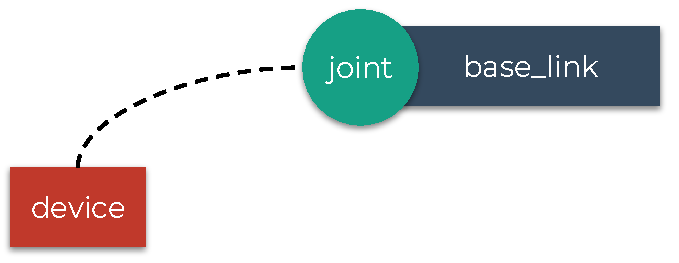
\includegraphics[width=.7\linewidth]{generalization/figures/squashing_transforms_desired.pdf}
  \caption{Webots' model representation}
  \label{fig:generalization:squashing_transforms:desired}
\end{subfigure}
\caption{Typical robot representation in \ac{urdf} and in Webots}
\label{fig:generalization:squashing_transforms}
\end{figure}

In the figure, there is Webots \texttt{Solid} node which got converted to \ac{urdf} link tagged as \texttt{Solid (no name)}. 
Although this may be desirable in some cases, it usually makes \ac{ros2} transform tree complex, which leads to unnecessary computations.
In order to avoid the computations, a squashing is performed.
It means that only relevant Webots nodes are exported into \ac{urdf} (as link nodes) while the others are neglected.
The relevant nodes are all nodes that have a \texttt{name} field defined.
The field \texttt{name} is always present for devices, and users can explicitly define \texttt{name} fields if it should be exported as a \ac{urdf} link.

As multiple intermediate Webots nodes can be neglected, the translation of child node ($I_0$) in respect to it's parent node ($I_N$) is defined as:
\begin{equation}
    \bm{T}_{I_0}^{I_N} = \sum_{i=0}^{N-1} \bm{T}_{I_i}^{I_{i+1}}
\end{equation}
whereas the translation of the intermediate node ($I_m$) in respect to it's parent ($I_n$) is represented by $ \bm{T}_{I_m}^{I_n} $ and consists of a three-dimensional vector.
Similarly, we do for the rotations:

\begin{equation}
    \bm{R}_{I_0}^{I_N} = \prod_{i=0}^{N-1} \bm{R}_{I_i}^{I_{i+1}}
\end{equation}
Note that $ \bm{R}_{I_0}^{I_N} $ is a $ 3 \times 3 $ rotation matrix and that the matrix multiplication has to be started from the parent.
In the implementation, a node recursively tries to find a relevant parent (visiting nodes towards the tree's root) while adding the visited nodes to the list.
Once the relevant node is reached, it calculates the translation from the first element in the list.

The rotation matrix has to be converted to Euler angles around a fixed axis (extrinsic) roll-pitch-yaw to match \ac{urdf}'s specification. This is done according to \cite[p. 9]{eberly_euler_nodate}.

Finally, the inter-process communication (from Webots simulation to Webots \ac{api}) is extended to support a new function:

\begin{minted}{c}
const char *wb_robot_get_urdf(const char *prefix);
\end{minted}

The \ac{api} function is exposed to C++, Python, MATLAB, Java and \ac{ros} client libraries.

\subsubsection{Utilization of robot\_state\_publisher}

Once the Webots' \ac{api} is capable of exporting \ac{urdf} as a string it can be utilized in the \ac{ros2} driver to publish \ac{ros2} transforms.
The approach to publish the transform is given in Figure \ref{fig:generalization:transforms_method_3}.

\begin{figure}[H]
    \centering
    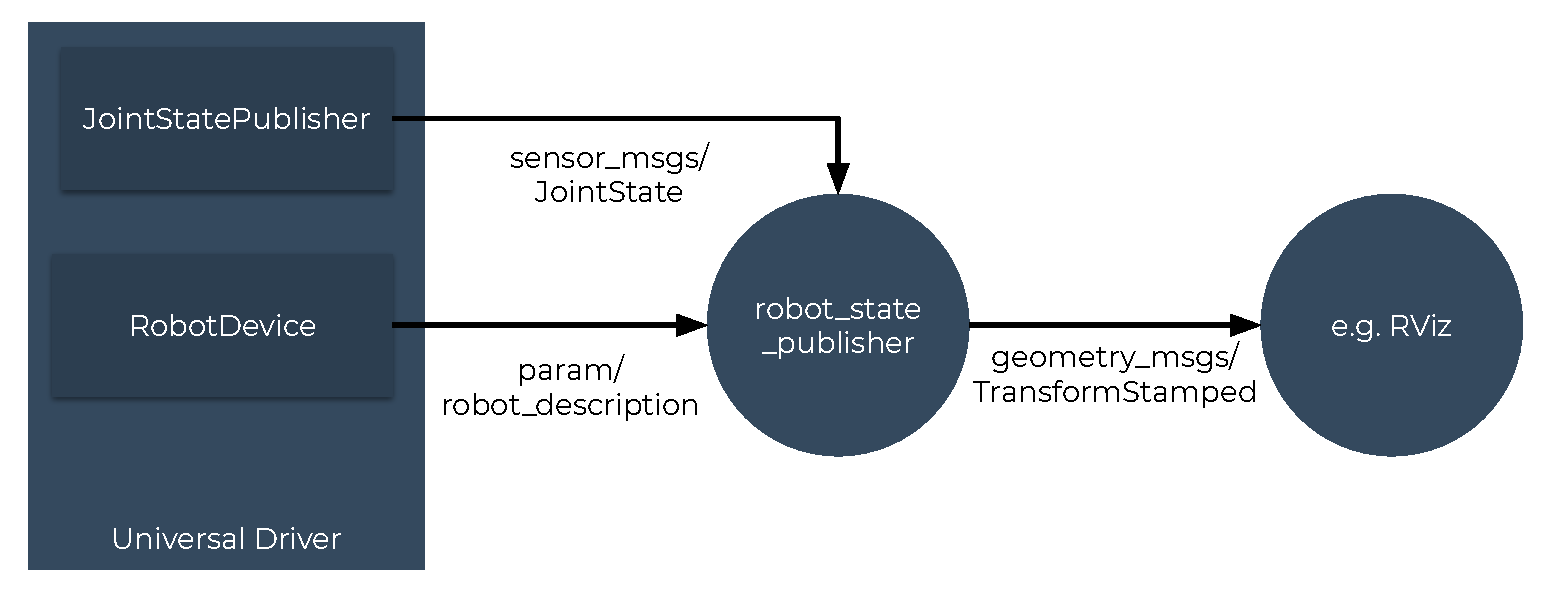
\includegraphics[width=\textwidth]{generalization/figures/transforms_method_3.pdf}
    \caption{Publishing \ac{ros2} transforms using \ac{urdf} and \texttt{robot\_state\_publisher}}
    \label{fig:generalization:transforms_method_3}
\end{figure}

In the figure, the universal driver has to provide the parameter \texttt{robot\_description} (\ac{urdf} string) and a topic with messages of type \texttt{sensor\_msgs/JointState} which contains readings from Webots \texttt{PositionSensor}s.
The parameter and the topic are consumed by \texttt{robot\_state\_publisher} (\ac{ros2} community node) which publishes \ac{ros2} transformations.

\section{\ac{ros2} Wrapped Devices}
As mentioned before, the universal driver is supposed to create \ac{ros2} automatically interface for each Webots device.
In the scope of this master project, modules that perform the conversion from Webots to \ac{ros2} interface are created for all Webots devices available on e-puck2, Khepera IV, and TurtleBot3 Burger.
The code is designed to be easily expandable to other Webots devices as well.

In this section, a brief explanation will be given for a few Webots devices.

\subsection{Differential Drive}
The differential drive module interacts with two motors and two position sensors.
The implementation is the same as explained in Section \ref{sec:simulation:odometry_velocity}, but it is decoupled from the rest of the driver to work as an independent component.
Also, it provides a high level of configurability (see table bellow, Table \ref{tab:generalization:diff_driver_params}).

\begin{table}[H]
    \centering
    \begin{tabular}{|l|l|}
        \hline
        \textbf{Name} & \textbf{Description} \\
        \hline
        \texttt{left\_encoder} & Name of position sensor mounted on the left wheel \\
        \hline
        \texttt{right\_encoder} & Name of position sensor mounted on the right wheel \\
        \hline
        \texttt{left\_joint} & Name of motor mounted on the left wheel \\
        \hline
        \texttt{right\_joint} & Name of motor mounted on the right wheel \\
        \hline
        \texttt{wheel\_distance} & Distance between left and right wheel in meters \\
        \hline
        \texttt{wheel\_radius} & Radius of the wheels \\
        \hline
        \texttt{command\_topic} & Topic name on which it should receive velocity commands \\
        \hline
        \texttt{odometry\_topic} & Topic name to which it should publish odometry data \\
        \hline
        \texttt{odometry\_frame} & Odometry frame name used in \ac{ros2} transform messages \\
        \hline
        \texttt{robot\_base\_frame} & Robot base frame name used in \ac{ros2} transform messages \\
        \hline
    \end{tabular}
    \caption{Parameters available for differential drive module}
    \label{tab:generalization:diff_driver_params}
\end{table}

\subsection{Range}
Webots returns value from distance sensors according to specified lookup table\footnote{In the example of lookup table first column represents the actual measurement, the second is the raw measurement, and the third column is the noise.}. 

\begin{minted}{python}
lookupTable [ 0     1000  0,
              0.1   200   0.1 ]
\end{minted}

It means it will not necessarily return a real distance to the closest object, but what Webots consider a raw value - linearly interpolated value.
Therefore, to obtain the actual distance, the lookup table has to be read.
The values are then interpolated according to the table.

However, Webots \ac{api} doesn't provide function to retrieve lookup table.
Therefore, the function is implemented\footnote{The \ac{api} function to obtained lookup table is also added for \texttt{Accelerometer}, \texttt{Compass}, \texttt{Gyro}, \texttt{InertialUnit}, \texttt{LightSensor} and \texttt{TouchSensor}.
All \ac{api} functions are also added to C, C++, Python, MATLAB, Java and \ac{ros}.} similarly to one explained in Section \ref{subsub:generalization:urdf_export}.

Then, in the universal controller, the actual values are returned, as shown by Algorithm \ref{fig:generalization:interopolation}.

\begin{figure}[H]
    \begin{minipage}{\linewidth}
    \begin{procedure}[H]
        return $ \frac{y_{end} - y_{start}}{x_{end} - x_{start}} (x_{value} - x_{start}) + y_{start}
 $ \;
        \caption{interpolate ($x_{value}$, $x_{start}$, $y_{start}$, $x_{end}$, $y_{end}$)}
    \end{procedure}
    \end{minipage}
    \begin{minipage}{\linewidth}
    \begin{procedure}[H]
        \For{$i\gets0$ \KwTo size of table $ T $ - 1}{
            \If{$(x_{value} T_{raw}[i] \land x_{value} \geq T_{raw}[i + 1]) \lor (
                x_{value} > T_{raw}[i] \land x_{value} \leq T_{raw}[i + 1])$}{
                return interpolate($x_{value}$, $T_{raw}[i]$, $T_{actual}[i]$, $T_{raw}[i+1]$, $T_{actual}[i+1]$) \;
            }
        }

        \tcc*{Extrapolation, assumes the table is sorted in descending order}

        \eIf{$x_{value} > T_{raw}[0] $}{
            return interpolate($x_{value}$, $T_{raw}[0]$, $T_{actual}[0]$, $T_{raw}[1]$, $T_{actual}[1]$) \;
        }{
            return interpolate($x_{value}$, $T_{raw}[-2]$, $T_{actual}[-2]$, $T_{raw}[-1]$, $T_{actual}[-1]$) \;
        }
        \caption{interpolateTable ($x_{value}$, $T$)}
    \end{procedure}
    \end{minipage}
\caption{Procedure used to interpolate table}
\label{fig:generalization:interopolation}
\end{figure}

Once actual values are obtained, the values are packed into messages of type \texttt{sensor\_msgs/Range} and published.

\begin{table}[H]
    \centering
    \begin{tabular}{|l|l|}
        \hline
        \textbf{Name} & \textbf{Description} \\
        \hline
        \texttt{topic\_name} & \ac{ros2} topic name \\
        \hline
        \texttt{timestep} & Publish period in ms  \\
        \hline
        \texttt{disable} & Whether to create \ac{ros2} interface for this sensor \\
        \hline
        \texttt{always\_publish} & Publish even if there are no subscribers \\
        \hline
        \texttt{frame\_id} & Value for \texttt{header.frame\_id} field \\
        \hline
    \end{tabular}
    \caption{Parameters available for distance sensor device}
    \label{tab:generalization:distance_params}
\end{table}

% TODO: \subsection{Camera}
% TODO: \subsection{\ac{lidar}}
